% Template for a Computer Science Tripos Part II project dissertation
\documentclass[12pt,a4paper,twoside,openright]{report}
\usepackage[pdfborder={0 0 0}]{hyperref}    % turns references into hyperlinks
\usepackage[margin=25mm]{geometry}  % adjusts page layout
\usepackage{graphicx}  % allows inclusion of PDF, PNG and JPG images
\usepackage{verbatim}
\usepackage{docmute}   % only needed to allow inclusion of proposal.tex
\usepackage{amsmath, amsfonts}

\raggedbottom                           % try to avoid widows and orphans
\sloppy
\clubpenalty1000%
\widowpenalty1000%

\renewcommand{\baselinestretch}{1.1}    % adjust line spacing to make
                                        % more readable

\begin{document}

\bibliographystyle{plain}


%%%%%%%%%%%%%%%%%%%%%%%%%%%%%%%%%%%%%%%%%%%%%%%%%%%%%%%%%%%%%%%%%%%%%%%%
% Title


\pagestyle{empty}

\rightline{\LARGE \textbf{Raahil Shah}}

\vspace*{60mm}
\begin{center}
\Huge
\textbf{MSMPTCP using Random Linear Network Coding} \\[5mm]
Computer Science Tripos -- Part II \\[5mm]
Churchill College \\[5mm]
\today  % today's date
\end{center}

%%%%%%%%%%%%%%%%%%%%%%%%%%%%%%%%%%%%%%%%%%%%%%%%%%%%%%%%%%%%%%%%%%%%%%%%%%%%%%
% Proforma, table of contents and list of figures

\pagestyle{plain}

\chapter*{Proforma}

{\large
\begin{tabular}{ll}
Name:               & \bf Raahil Shah                       \\
College:            & \bf Churchill College                     \\
Project Title:      & \bf MSMPTCP using Random Linear Network Coding \\
Examination:        & \bf Computer Science Tripos -- Part II, May 2016  \\
Word Count:         & \bf 0\footnotemark[1]
                      (well less than the 12000 limit)  \\
Project Originator: & Dr J. Crowcroft                    \\
Supervisor:         & Dr J. Crowcroft                    \\ 
\end{tabular}
}
\footnotetext[1]{This word count was computed
by \texttt{detex diss.tex | tr -cd '0-9A-Za-z $\tt\backslash$n' | wc -w}
}
\stepcounter{footnote}


\section*{Original Aims of the Project}

The original aim of this project was to combine Multipath TCP (MPTCP) with the Network Coding paradigm while allowing for many-to-one flows, i.e. multiple sources. While Multipath TCP provides greater resource usage and often near optimal load balancing by spreading information across multiple flows, the addition of network coding, by spreading information over both packets and flows, aims to maximise the degrees of freedom available from resource pooling. The protocol was to be testing on simulated wireless topologies in a network simulator to evaluate its performance in terms of throughput and robustness against failures. 

\section*{Work Completed}

In this project I provide a simple design and implementation of network coding using the random linear network coding technique. The coding layer is run in the chosen network simulator: ns-3 using the Kodo library for C++ and ns3. Due to challenges (mentioned below) the network coding is run over UDP, rather than MPTCP, in the application layer. The simulations achieve reliable file transfer over UDP and increased reliable throughput over lossy wireless channels.

%TODO include eval

\section*{Special Difficulties}

After researching MPTCP and MPTCP with network coding (MPTCP/NC) protocols, implementing the multisource and network coding extensions seemed too ambitious, especially in the time frame of this project. Further, the main challenge with using MPTCP for this project was the lack of a publicly available MPTCP module implemented for ns3. In consultation with my supervisor and the overseers I decided to follow the backup strategy laid out in the proposal [Appendix \ref{ch:proposal}] which was to use the coding layer over UDP instead of MPTCP. 
 
\newpage
\section*{Declaration}

I, Raahil Shah of Churchill College, being a candidate for Part II of the Computer
Science Tripos, hereby declare
that this dissertation and the work described in it are my own work,
unaided except as may be specified below, and that the dissertation
does not contain material that has already been used to any substantial
extent for a comparable purpose.

\bigskip
\leftline{Signed }

\medskip
\leftline{Date }

\tableofcontents

\listoffigures

\newpage
\section*{Acknowledgements}


%%%%%%%%%%%%%%%%%%%%%%%%%%%%%%%%%%%%%%%%%%%%%%%%%%%%%%%%%%%%%%%%%%%%%%%
% now for the chapters

\pagestyle{headings}

\chapter{Introduction} \label{ch:intro}

\section{Motivation for the Project}

The widespread success and rapid growth of wireless technologies in communication networks make it clear that wireless networking is closely linked to the present and future of communications. However, the Transmission Control Protocol (TCP) presently used in a wide variety of applications for reliable data transfer, suffers greatly in performance from the challenges presented by today's wireless networks. These include the multipath nature of networks, for example with devices having multiple wireless interfaces, datacenters having redundant paths and large server farms employing multihoming, as well as the lossy nature of wireless links resulting in the need for complex management schemes in the protocol to ensure reliable transmission. Recent research work shows that these challenges can be addressed by the the concept of network coding, originally introduced by Ahlswede et al. \cite{ahlswede}, and the new Multipath TCP (MPTCP)\cite{mptcp-ietf}, an ongoing effort of the Internet Engineering Task Force (IETF) MPTCP working group.

Network Coding is a field of information theory that presents an alternative to the conventional store-and-forward routing paradigm and allows us to extend existing resource pooling from information streams sharing network resources to spreading the information over the data packets as well. Using network coding, nodes can modify the data of the packets across the network, either at the source or at an intermediate node (router) which can lead to a number of performance benefits, including reducing the number of transmissions needed for a reliable transfer providing increased throughput, increasing robustness to packet losses and link failures as well as potential implicit security mechanisms from the transmission of coded rather than raw packet data. Summarised developments on network coding and its benefits can be found in \cite{nc-intro}.

MPTCP is a major modification of TCP that allows a single transport layer connection to use multiple paths simultaneously. It's application can be seen in many real world scenarios, for example a cell phone or laptop with multiple network interfaces (WiFi/3G) downloading a file. MPTCP allows the device to set up multiple `subflows' for a single MPTCP session. This not only leads to better load balancing across the flows which significantly benefits throughput especially for lossy wireless networks like WiFi and 3G, but also results in smoother handover in the case that one of the interfaces goes down as compared to an application layer handover over TCP. \cite{mptcp-over} presents a succinct overview of the implementation and performance of the protocol.  

Several suggestions on combining network coding with MPTCP or TCP have been proposed in literature (\cite{mptcp-nc-mesh}, \cite{mptcpnc}, \cite{tcpnc}). They indicate that MPTCP/NC provides better throughput, robustness to packet losses and scheduling of packets on each subflow, under certain experimental conditions and assumptions. These results are enough to show us that integrating network coding in today's protocol stack has great potential to strengthen and enhance wireless communications. 

\section{Project Description}

%TODO: Include eval

This project successfully demonstrates the benefits of network coding with respect to reliable transfer, throughput gain and robustness to packet losses on wireless networks. This is achieved by implementing a simple network coding protocol which is described in Section \ref{sec:nclayer}. The protocol is demonstrated to run in the application layer of the OSI protocol stack over a standard, real world network stack comprising of User Datagram Protocol (UDP) in the transport layer, Internet Protocol version 4 (IPv4) in the network layer and ad hoc 802.11 WiFi in the link and physical layers. 

The network coding scheme implemented is Intra-flow network coding using Random Linear Coding (RLC), discussed in Section \ref{sec:nctheory}, which mixes or codes datagrams from the same UDP flow. The coding layer is used to implement two techniques of Intra-flow network coding:
\begin{description}
 	\item[Random Linear Source Coding] where only the source node(s) code the original (native) packets to transmit a sequence of coded packets into the network while the intermediate nodes simply relay the coded packets received onwards using the conventional store-and-forward paradigm.
 	\item[Random Linear Network Coding] where along with RLC at the source node(s), the intermediate relay nodes may perform `re-coding' operations on the coded packets received, forwarding new coding packets to the next hop in the network.
 \end{description}
 The performance of each technique is evaluated in Sections \ref{sec:rlsc}, \ref{sec:rlnc}. We also look at the effects of varying the RLC parameters of the size of the Galois Field used to select coding coefficients and the size of the generation (block of naive packets) used for coding at the source in Section \ref{sec:fieldgen}.

 The network coding protocol implementation and evaluation is performed in ns-3 (specifically ns-3.25), a widely used discrete event network simulator publicly available under the GNU GPLv2 license for research and development \cite{ns3}. Along with ns-3 I integrated and used Kodo \cite{kodo}, a commercial network coding library developed by Steinwurf, which provides a highly optimised API for RLC operations. Its use for this project is discussed in Section \ref{sec:kodo}.

 The work done in this project can be easily extended for a variety of applications and simulation scenarios in ns-3, including running the coding layer over TCP or MPTCP implementations, running network coding under the transport layer (as in \cite{gomez}) and implementing the Inter-flow network coding technique (also seen in \cite{gomez}).


\chapter{Preparation} \label{ch:prep}

\section{Requirements Analysis} \label{sec:start}

The requirements to undertake the project were as follows:
\begin{description}
	\item[Theory] The project required a strong understanding of computer networking from both a mathematical and engineering perspective; the former to grasp the concept of linear network coding and the latter to understand its application and use with existing networking protocols. My starting point for the theoretical background was a knowledge of principles and protocols of modern computer networks from Part 1B of the course. 
	\item[Implementation] I had little prior experience with network programming (limited to socket programming in Java) and a basic proficiency with C++. For the implementation I had to meet the requirements of familiarising myself with network programming in C++. Further, I had to gain familiarity with the Kodo network coding library and its C++ APIs. 
	\item[Simulation] A major requirement for this project was a strong working proficiency with ns-3 from a user and developer's perspective. This included learning to use the Python based Waf build system, learning to use various ns-3 modules' APIs and understanding the ns-3 code base structure, in order to build a simple network coding module and API for ns-3 and write and run several simulations on varied network topologies.
	\item[Software Development] The software was required to be written mostly in C++ with some Python. For a version control strategy, Git and GitHub were used. The project files were regularly backed up on cloud storage and an external disk. Appendix \ref{ch:proposal} details the development requirements further.
\end{description}

\section{Network Coding Theory} \label{sec:nctheory}

\subsection{Relevant Research}

This first step in preparation was to read the literature on network coding theory, in specific on linear network coding. Ahlswede et al.\cite{ahlswede}'s seminal paper describes the multicast problem and main network coding theorem which shows that with network coding, a source can multicast information at a rate approaching the smallest minimum cut between the source and any receiver as the symbol size approaches infinity. Fragouli et al.\cite{nc-fund} detail a theoretical framework for network coding using a mathematical model to describe the relevant theorems, the analytic throughput benefits and the design of network coding algorithms. In \cite{tcpnc} an implementation of linear network coding with TCP as a modified TCP/NC protocol is explained.

\subsection{Linear Network Coding}

Let us consider an information relay body in a network, such as a router or node in an ad hoc network. Conventionally when this node receives a packet, it will store the packet and subsequently forward the packet to some other node in its original form. The network coding paradigm allows the node to combine a certain number of received packets to create one or many `coded' outgoing packets. 

Let us assume each packet is of size $L$ bits (or padded to $L$ bits). For a chosen positive integer $q$, each $L$ bit packet can be represented as a vector in the Galois Field $\mathbb{F}_q$, containing $L/s$ symbols where $s = \log_2 q$. We can consider each block of $s$ bits in the packet to be a symbol over $\mathbb{F}_q$. With linear network coding, we combine a set of $g$ (called a generation) many such packets to form the coded data $X \in {\mathbb{F}_q}^{L/s}$ with the coefficients are chosen from the $\mathbb{F}_q$ field and addition and multiplication is also performed over $\mathbb{F}_q$. The vector $c$ of $g$ coding coefficients used to compute $X$ is called the `encoding vector' or `coding vector'. A coded packet $(c, X)$, containing both the coding vector and the coded data is then sent on in the network. A destination node can decode a set of coded packets to retrieve the original packets once it has $g$ encoded packets with linearly independent encoding vectors. There are different algorithms used to select the coding coefficients used in encoding operation. These can be centralised or decentralised, as well as deterministic or randomised. The simple algorithm of selecting coefficients uniformly at random over $\mathbb{F}_q$ is called Random Linear Coding which is the technique I have used in this project. 

% TODO: fill maths?

\subsubsection{Throughput Gain}

\begin{figure}[tbh]
	\centerline{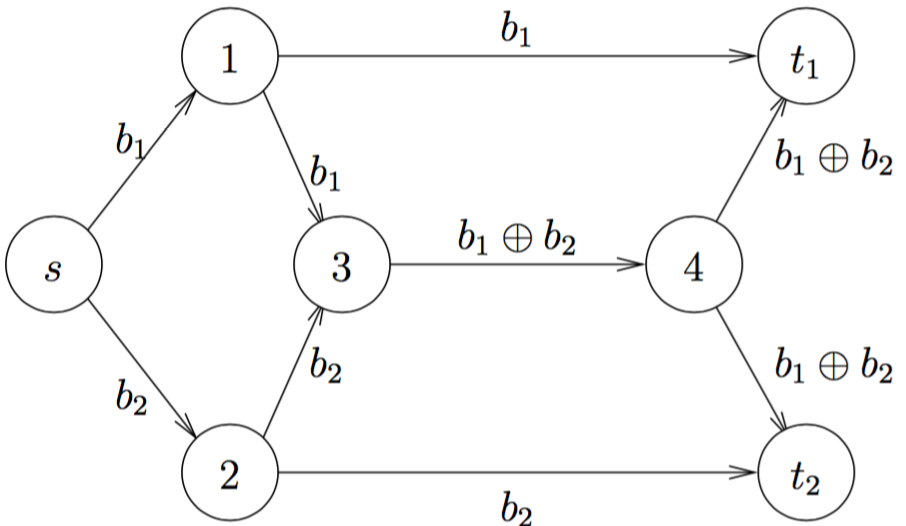
\includegraphics[scale=0.9]{figs/butterfly}}
	\caption{Butterfly network topology illustrating the throughput gain obtained by using linear network coding.\cite{nc-intro}}
	\label{fig:butterfly}
\end{figure}

To see the throughput gain using linear network coding, we consider the canonical Butterfly Network Topology example as seen in figure \ref{fig:butterfly}. Here source node $s$ aims to send sends two packets $b_1$ and $b_2$ to each of the sink nodes $t_1$ and $t_2$. Each arc is directed, reliable and has a capacity $1$. The operation of interest is performed at node $3$ which instead of simply relaying either one of $b_1$ or $b_2$, linearly combines the two received packets to form the coded packet $b_1 \oplus b_2$ and sends that to node $4$. Note here that this is linear network coding in the binary field $\mathbb{F}_2$. Sink $t_1$ receives packets $b_1$ and $b_1 \oplus b_2$, which are encoded packets with encoding vectors $(1, 0)$ and $(1, 1)$ respectively. As they are linearly independent, $t_1$ has all the information it needs to perform a decode to obtain the original packets by performing once addition in $\mathbb F _2$ as $b_2 = b_1 \oplus (b_1 \oplus b_2 )$. Similarly node $t_2$ can obtain both the original packets using $b_1 = b_2 \oplus (b_1 \oplus b_2 )$. Using linear coding, $s$ was able to multicast both packets to both sinks in a total of $9$ transmissions across the network. However if we were simply using routing, this would only be achieved with at least 2 more transmissions (at node $3$ and $4$).

\subsubsection{Robustness to Packet Losses}

\begin{figure}[tbh]
	\centerline{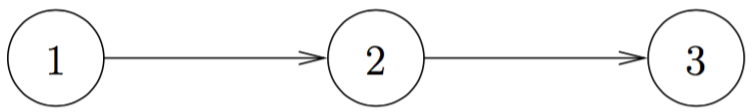
\includegraphics[scale=0.9]{figs/tandem}}
	\caption{Two link tandem network topology.\cite{nc-intro}}
	\label{fig:tandem}
\end{figure}

To see why network coding is useful in combating against packet losses we consider topology shown in figure \ref{fig:tandem}, with source node $1$ connected to the sink node $3$ via an intermediate node $2$. We can model erasure channels by considering the probability of packet loss on link $1 \rightarrow 2$ as some $\varepsilon_{12}$ while that on link $2 \rightarrow 3$ as some $\varepsilon_{23}$. In this packet loss model, the channel capacity of the $1 \rightarrow 2$ link is $\varepsilon_{12}$ packets per unit time that of the $2 \rightarrow 3$ link is $\varepsilon_{23}$ packets per unit time.Between nodes $1$ and $3$ we essentially have an erasure channel with erasure probablity $1 - (1 - \varepsilon_{12})(1 - \varepsilon_{23})$ with a capacity of $(1 - \varepsilon_{12})(1 - \varepsilon_{23})$. 

With no network coding we can send data from source to sink with a throughput of $(1 - \varepsilon_{12})(1 - \varepsilon_{23})$ packets per unit time. However the transmission is unreliable as packets lost at either link cannot be recovered at the sink. Employing network coding at the source, we introduce a degree of redundancy at the packet level, due to which even if only a subset of the packets sent from the source are received at the sink, the original data can be recovered, providing us reliable, in order transmission over the erasure channel. However, this reliability is achieved at a cost in throughput, which we can deduce using the result derived in Appendix \ref{app:bound}: To reliably send a block of $g$ packets using RLC at the source, the source node will on average have to transmit at most:
\[ 
\frac{g + 1.607}{(1 - \varepsilon_{12})(1 - \varepsilon_{23})}
\]
total coded packets.

It is interesting to note that network coding can be applied at the intermediate node $2$ as well, if the intermediate node is equipped with the coding protocol. In this scheme node $2$ decodes the packets it receives and then recodes the packets before communicating them onward to node $3$. Using intermediate node recoding we can communicate over the $1 \rightarrow 2$ link at a rate of $1 - \varepsilon_{12}$ packets per unit time and over the $2 \rightarrow 3$ link at $1 - \varepsilon_{23}$ packets per unit time, and so communicate between nodes $1$ and $3$ at a increased rate of $\min (1 - \varepsilon_{12}, 1 - \varepsilon_{23})$. In practice network coding at intermediate nodes has its drawbacks in particular the resultant increase in delay due to the computational task of decoding and recoding at each hop in the network. 

\section{Network Protocols: MPTCP, TCP/NC, UDP}

\section{Network Simulator: ns3}

\chapter{Implementation} \label{ch:imp}

\section{Network Coding Layer} \label{sec:nclayer}

\subsection{Protocol Description}

The network coding layer is implemented as an ns-3 module and is used in the application layer for coding simulations. The protocol is designed to be as simple as possible with the aim of providing a network coding layer with minimal modification to the current networking stack and minimal data and computation overhead. Figure \ref{fig:proto-overview} presents an overview of the core high level operations involved in the network coding protocol. 

\begin{figure}[tbh]
	\centerline{\includegraphics[scale=0.7]{figs/proto-overview}}
	\caption{Network coding layer protocol overview.}
	\label{fig:proto-overview}
\end{figure}

At a coding node (source or intermediate), the generation of $L$ bit packets to be coded are passed to an encoder object. In the encode step, the encoder generates an $L$ bits of coded data and $g$ bits of the coding vector used. This is encapsulated as a coded data packet and transmitted from the node. On the receiver end, a coded data packet is unpacked and the coding vector and coded data are passed to the decoder. When the decoder has received $g$ innovative coded packets, it is able do perform a decode operation to obtain the $g$ original packets. The node that has performed a decode then generates an $ACK$ acknowledgement packet which is sent back to the source to acknowledge the successful reception of the generation.

\subsection{Coding Parameters}


The coding layer RLC implementation is designed to be as general as possible, by allowing the encoders and decoders to be configured with different RLC parameters. This is to allow for a variety of simulation scenarios, to be able to evaluate the effects performance from varying the parameters and make the code extensible.

In the background on RLC theory provided in Section \ref{sec:nctheory}, we introduced the three coding parameters: field size $q$, generation size $g$ and packet length $L$. In this section we will discuss their practical relevance to the coding protocol implementation.

\begin{description}
	\item[Field size $q$] is the size of the Galois Field from which the coding coefficients is selected. From the analytical results in Appendix \ref{app:bound}, we can see that increasing $q$ rapidly increases the probability of obtaining uniformly selected coding vectors that are linearly independent. The trade off for using higher field sizes is that it leads to larger memory requirements and increased computation time for the finite field computations. Each coding node's memory requirements $O(\log q)$, logarithmic in the field size.

	  Commonly used values for $q$ include $2$ and $8$ as they correspond to bit and byte sized field elements respectively. The coding layer implementation allows for $3$ different field sizes, $q = 2, 4, 8$.
	\item[Generation size $q$] is the size of the block of original packets that are encoded together. Only packets of the same generation are coded together. The size and composition of generations may have significant impact on the performance of network coding\ref{sec:fieldgen}. The analysis in Appendex \ref{app:bound} shows that like $q$, an increase in $g$ increases the likelihood of linearly independent coding vector selection and consequently reduces the expected number of additional packets that need to be encoded. 

	However the memory requirement of a coding node increases quadratically, $O(q^2)$, with increase in generation size. Increasing the value of $g$ also increases the complexity of encoding and decoding computations. 

	My coding protocol allows arbitrary selection of the generation size. 
	\item[Packet size L] determines the `breadth' of each generation block. $L$ does not affect the RLC algebra, but it does change the dimension of the vector space of original and coded packets. The memory requirement at a node increases linearly with an increase in $L$.

	Packet size can be varied arbitrarily when setting up the coding protocol.

\end{description}

\subsection{Packet Format} \label{sec:pack}
For the coding protocol I designed a simple custom packet format to encapsulate the packets generated at this layer. Figure \ref{fig:packet} shows the general structure of the new coding layer packet.

\begin{figure}[tbh]
	\centerline{\includegraphics[scale=0.65]{figs/packet}}
	\caption{Network coding protocol packet structure for data and ACK packets.}
	\label{fig:packet}
\end{figure}

\begin{description}
	\item[Packet Type] This is a 1 bit field that denotes whether a packet is a data packet, i.e. containing a RLC coded data packet, or an ACK packet used to acknowledge a successfully decoded generation of packets.
	\item[Coding Header] This is a varying size field that contains, among other fields, a representation of the coding vector for the coded packet. The size of the coding vector and therefore the coding header depends on $q$ and $g$. The exact format of the coding header is a low level implementation detail of the Kodo coding library \cite{kodo} which used I have built upon for the encoding and decoding modules.
	\item[Coded Packet Data] This payload is the linearly coded packet data formed using the coding vector present in the coding header. 
\end{description}

\subsection{Encoding}

\subsubsection{Source Encoding Algorithm}
To encode a generation of original packets, $M_1, M_2, ..., M_g$, the encoder first stores the original symbols in a $g \times L / \log_2 q$ matrix. To generate a coded packet $X_i$, the encoder picks $g$ coding coefficients from a uniform random distribution over $\mathbb{F}_q$, to form the $g$ dimensional coding vector $c_j$. The coded packet data is computed using finite field operations over $\mathbb{F}_q$ as:
\begin{equation}
	X_i = \sum_{j = 0}^g (c_i)_j M_j
\end{equation}

This coded data $X_i$ is then combined with the coding vector $c_i$ as well as the Packet Type($= 1$ for data packet) as described in Section \ref{sec:pack}, to form a coding protocol layer packet. This packet is then sent to the next node. At this node we also schedule a call to the next send, to perform the next encoding and transmission, at a future time based on a predetermined packet transmission interval, only if we have not received an ACK from the receiver indicating that the it has received sufficient packets to decode the generation. In this was a coding node repeatedly sends coded transmissions, until the decoder has sufficient information to decode them. This simple code-and-send-until-ack strategy allows us to reliably transfer and acknowledge $g$ packets from source to destination, on lossy and lossless channels. Further, in the case that the ACK is lost due to packet loss, the protocol adapts by default to retry as the sender, unaware that the receiver has successfully received $g$ innovative packets needed for decoding, will send another coded packet from the generation which the decoder will deem redundant and reply with an ACK.

\subsubsection{Recoding Algorithm}
Recoding is the technique of recursively applying RLC at the node in the next hop of the network. An intermediate recoding node, which has received a set of $m$ encoded packets, $(c_1, X_1), ..., (c_m, X_m)$, can generate a new recoded packet $(e, Y)$ by first picking an $m$ dimensional random coding vector $d = (d_1, ..., d_m)$ to compute the recoded data as:
\begin{equation}
	Y = \sum_{i = 0}^m d_i (X_1)
\end{equation}

This recoded data is still a linear combination of the original packets:
\begin{equation}
	Y = \sum_{i = 0}^m d_i \sum_{j = 0}^g (c_i)_j M_j
	= \sum_{j = 0}^g \left(\sum_{i = 0}^m d_i (c_i)_j \right) M_j
\end{equation}

The coding vector for the recoded packet is then calculated as:
\begin{equation}
	e = \sum_{i = 0}^m d_i (c_i)_j
\end{equation}

Finally the recoded packet $(e, Y)$ can be transmitted. Using the network coding layer, recoding can be performed at any node in the network however the nodes must be within a single flow (Intra-flow network coding) as only then will the packets be guaranteed to have been encoded from the same generation.

\subsubsection{Memory Requirements}
To perform the encoding operation, an encoding node (source or intermediate recoding node) requires a generation block $g \times L$ bits of memory to store the data to be encoded and a $g \times g \times \log_2 q$ bit block of memory to store the coding matrix of coefficients used. 

In my implementation, I allocate an $g \times L$ block size encoder buffer to store the symbols to be encoded. The Kodo library encoder object handles the storage and representation of the coding coefficients. Once a generation has been successfully transmitted to the decoder, the next $g \times L$ block is passed into the buffer to code the next generation. 

\subsection{Decoding}

\subsubsection{Decoding Algorithm}

The decoding module is implemented for the receiver side of the protocol. When a node receives a coding layer packet, it is first unpacked to inspect the packet type. An ACK packet is handled by the sender side of the node to load the next block packets to be encoded, and requires no implementation on the decoding side. A data packet payload which is some coded packet $(c_i, X_i)$, is passed to the decoder object, which if has not already successfully decoded the generation, will proceed to perform a decode operation with the new coded packet. 

The decoder can first compute whether the received coded packet is innovative by performing a rank calculation on the $g \times g$ coding matrix $C$ containing the linearly independent previously received coding vectors and the newly inserted $c_i$. If $c_i$ does not increase the rank of the matrix it must be linearly dependent on the other coding vectors and the packet $(c_i, X_i)$ is deemed non-innovative and discarded. However if the packet is innovative the decoder stores $c_i$ in the coding matrix and $X_i$ in the $g \times L / \log_2 q$ data/symbol matrix $X$. 

Once $g$ such innovative packets have been received, the decoder can then calculate the $g \times L / \log_2 q$ matrix of original symbols $M$ as:
\begin{equation}
	M = C^{-1} \times X
\end{equation}

The matrix equation is then solved using Gaussian elimination, which is performed by the Kodo decoder object.

\subsubsection{Memory Requirements}

Similar to the encoder module, the decoder requires a $g \times L$ bit buffer to store the coded packet data received and a $g \times g \times \log_2 q$ bits to store the coding matrix. Note that the decoder does not need to store all the coded data and coding vectors received because it can dynamically discard packets with linearly dependent coding vectors. 

In my implementation a $g \times L$ bit block size decoder buffer is allocated to the Kodo decoder object. After the decoder has successfully performed elimination on the coding matrix and decoder data buffer, the data buffer is left with the original packets of the generation, in order.

\section{Simulation in ns-3} \label{sec:ns3}

\section{Kodo Network Coding Libary} \label{sec:kodo}

\section{Reliable Transfer over UDP}

\chapter{Evaluation} \label{ch:eval}

\section{Reliable File Transfer} \label{sec:relUDP}

\section{Varying Field and Generation Size} \label{sec:fieldgen}

\section{Random Linear Source Coding} \label{sec:rlsc}

\section{Random Linear Network Coding} \label{sec:rlnc}

\chapter{Conclusion} \label{ch:conc}

%%%%%%%%%%%%%%%%%%%%%%%%%%%%%%%%%%%%%%%%%%%%%%%%%%%%%%%%%%%%%%%%%%%%%
% the bibliography
\addcontentsline{toc}{chapter}{Bibliography}
\bibliography{refs}

%%%%%%%%%%%%%%%%%%%%%%%%%%%%%%%%%%%%%%%%%%%%%%%%%%%%%%%%%%%%%%%%%%%%%
% the appendices
\appendix

\chapter{Project Proposal}
\label{ch:proposal}

% Note: this file can be compiled on its own, but is also included by
% diss.tex (using the docmute.sty package to ignore the preamble)
\documentclass[12pt,a4paper,twoside]{article}
\usepackage[pdfborder={0 0 0}]{hyperref}
\usepackage[margin=25mm]{geometry}
\usepackage{graphicx}

\renewcommand\labelitemi{--}

\begin{document}

\vfil

\centerline{\Large Computer Science Project Proposal}
\vspace{0.4in}
\centerline{\Large MSMPTCP: Multisource Multipath TCP using Random Linear Codes}
\vspace{0.4in}
\centerline{\large R. Shah, Churchill College}
\vspace{0.3in}
\centerline{\large Originator: Dr J. Crowcroft}
\vspace{0.3in}
\centerline{\large \today}

\vfil

\noindent
{\bf Project Supervisor:} Dr J. Crowcroft
\vspace{0.2in}

\noindent
{\bf Director of Studies:} Dr J. K. Fawcett
\vspace{0.2in}
\noindent
 
\noindent
{\bf Project Overseers:} Dr T. G. Griffin  \& Dr P. Lio'


% Main document

\section*{Introduction, The Problem To Be Addressed}
MPTCP is an extension to TCP that sprung from the observation that modern networks are quite often multipath, as seen in server farms that use multihoming, datacenters with several redundant paths between servers and in modern host devices such as mobile devices that have multiple network interfaces (for example, WiFi and 3G). TCP by itself cannot take advantage of this to load balance across multiple paths. MPTCP, on the other hand, allows for multiple subflows to be set up for a single session, reaping the benefits of resource pooling using multiple paths in the network, all transparent to the application. \cite{mptcp}

This project aims to extend MPTCP, to incorporate network coding and to allow for multiple sources for the connection. Adding multisourcing to MPTCP has its advantages in cases where there is a lot of replication of data, for example within and across many datacenters. The addition of network coding to MPTCP spreads information over both packets and flows, maximising the degrees of freedom that resource pooling can enjoy. Further network coding can increase throughput and improve robustness against failures, especially in lossy networks (for example, wireless networks). \cite{nc-tcp}

\section*{Starting Point}

This project will build on an existing userspace implementation of MPTCP to extend it to MSMPTCP with random linear coding.

\section*{Resources Required}

\begin{description}
  \item[Hardware] Personal computer: MacBook Pro (Mid 2014), 8GB 1600 MHz DDR3 RAM, 2.8 GHz Intel Core i5 Processor, running Mac OS X 10.11.
  \item[Software] Network Simulator (ns-2 or ns-3).
  \item[Backup] All the project files, i.e. source code, research and authored documents, will be stored under a project directory on my personal computer which is synced to cloud storage (Google Drive). For an offline solution, the project directory will be backed up (with at least weekly frequency) to an external hard disk using Time Machine. I will also maintain (at least weekly updated) a backup of the project directory on the university MCS to be used in case my personal machine cannot be used for project work. I would require an extension of storage space on the MCS for this purpose. All source code and written documents will be under git version control and pushed to a private repository on GitHub. Commits and pushes will be made at least daily and each time a significant change to any code or document is made. 
\end{description}

\section*{Work to be done}

The project breaks down into the following sub-projects:

\begin{enumerate}
  \item Implementing a network coding layer using random linear codes. This will involve implementing a sender side coding module and a receiver side decoding module. The coding implementation will be tested on the standard butterfly network topology in the network simulator. 
  \item Extending MPTCP to MSMPTCP with network coding. This sub-project will involve extending the MPTCP implementation to include the network coding layer implemented in sub-project 1 along with adding support for multiple sources. The resulting MSMPTCP implementation will be tested in the network simulator on a butterfly topology with multiple sources. In case extending MPTCP proves unfeasible within the time frame of this project, the fallback task for this sub-project would be to add the multisource and network coding extensions to a simpler base protocol such as UDP. The fallback protocol will be tested for the same cases as MSMPTCP and the same success criterion for the sub-project will apply.
  \item Evaluating the performance of MSMPTCP with network coding against MPTCP and TCP. The evaluation will take the form of graphs of throughput obtained for MSMPTCP with random linear codes against that obtained for MPTCP and TCP, for tests run on the network simulator. Performance of MPTCP and MSMPTCP could also be compared for varying number of subflows. 
\end{enumerate}

\section*{Success Criterion for the Main Result}

The success criterion for sub-project 1 would be a set of successful tests of the implemented network coding layer in the network simulator on the standard butterfly topology. Similarly, sub-project 2 can be considered successful if the MSMPTCP with network coding implementation succeeds for a set of network simulator tests on the standard butterfly topology along with a butterfly topology with multiple sources. 

\section*{Possible Extensions}

\begin{enumerate}
  \item Re-encoding packets at intermediate nodes which is useful in combating against packet losses.
  \item Testing MSMPTCP with random linear coding with various different network topologies in network simulator.
\end{enumerate}

\section*{Timetable: Workplan and Milestones to be achieved.}

Planned starting date is 22/10/2015.

\begin{enumerate}

\item {\bf Michaelmas weeks 3, 4} (22/10/2015 - 04/11/2015)

Research on network coding theory with specific focus on random linear codes and implementations of network coding with TCP.
\begin{itemize}
  \item {\em Deliverable:} Summary of theory learned and an implementation strategy for random linear coding in a LaTeX document for inclusion in the progress report. 
  \item {\em Milestone:} Submit the deliverable document to supervisor for review and feedback.
\end{itemize}

\item {\bf Michaelmas weeks 5, 6} (5/10/2015 - 18/11/2015)
Install ns-2/ns-3 and learn to use it to generate network topologies and simulate protocols.

\begin{itemize}
  \item {\em Deliverable:} Simulation code and results for demo topologies and protocols.
  \item {\em Milestone:} Demonstrate topology generation and simulations to supervisor.
\end{itemize}

\item {\bf Michaelmas weeks 7, 8} (19/11/2015 - 02/12/2015)

Work on random linear coding implementation for sub-project 1.
\begin{itemize}
  \item {\em Deliverable:} Source code and documentation.
  \item {\em Milestone:} Unit test all code modules written.
\end{itemize}

\item {\bf Michaelmas vacation weeks 1, 2} (03/12/2015 - 16/12/2015)

Work on random linear coding implementation for sub-project 1.
\begin{itemize}
  \item {\em Deliverable:} Source code and documentation.
  \item {\em Milestone:} Unit test all code modules written. Have a feature complete network coding layer implementation.
\end{itemize}

\item {\bf Michaelmas vacation weeks 3, 4} (17/12/2015 - 30/12/2015)

Test the network coding layer on the standard butterfly topology in network simulator.
\begin{itemize}
  \item {\em Deliverable:} Simulation code and results.
  \item {\em Milestone:} Have a tested, feature complete network coding layer implementation.
\end{itemize}

\item {\bf Michaelmas vacation weeks 5, 6} (31/12/2015 - 13/01/2015)

Slack time to complete any outstanding work for sub-project 1 and/or work on possible extensions.
Write the progress report. 
\begin{itemize}
  \item {\em Deliverable:} Draft progress report.
  \item {\em Milestone:} Have completed sub-project 1. Submit the draft progress report to supervisor and DoS for review and feedback.
\end{itemize}

\item {\bf Lent weeks 1, 2} (14/01/2016 - 27/01/2016)

Research on MPTCP and get familiar with the MPTCP implementation code.
\begin{itemize}
  \item {\em Deliverable:} Summary of research done and outline to extend MPTCP in a document.
  \item {\em Milestone:} Submit the deliverable document to supervisor for review and feedback. Submit the final progress report.
\end{itemize}

\item {\bf Lent weeks 3, 4} (28/01/2016 - 10/02/2016)

Work on MSMPTCP implementation for sub-project 2 using the network coding layer implementation from sub-project 1.
\begin{itemize}
  \item {\em Deliverable:} Source code and documentation.
  \item {\em Milestone:} Successful unit tests for any code modules written.
\end{itemize}

\item {\bf Lent weeks 5, 6} (11/02/2016 - 24/02/2016)

Work on MSMPTCP implementation for sub-project 2 using the network coding layer implementation from sub-project 1.
\begin{itemize}
  \item {\em Deliverable:} Source code and documentation.
  \item {\em Milestone:} Successful unit tests for any code modules written. Have a feature complete MSMPTCP implementation.
\end{itemize}

\item {\bf Lent weeks 7, 8} (25/02/2016 - 09/03/2016)

Test the MSMPTCP protocol with standard and multiple source butterfly topology in network simulator.
\begin{itemize}
  \item {\em Deliverable:} Simulation code and results.
  \item {\em Milestone:} Have a tested, feature complete MSMPTCP with random linear coding implementation.
\end{itemize}

\item {\bf Easter vacation weeks 1, 2} (10/03/2016 - 23/03/2016)

Slack time to complete any outstanding work for sub-project 2 and/or work on possible extensions.
\begin{itemize}
  \item {\em Milestone:} Have completed sub-projects 1 and 2.
\end{itemize}

\item {\bf Easter vacation weeks 3, 4} (24/03/2015 - 06/04/2015)

Work on drafting the main chapters of the dissertation.
\begin{itemize}
  \item {\em Deliverable:} Draft dissertation chapters.
  \item {\em Milestone:} Submit the draft to supervisor and DoS for review and feedback.
\end{itemize}

\item {\bf Easter vacation weeks 5, 6} (07/04/2015 - 20/04/2015)

Work on revising and completing draft dissertation incorporating feedback from supervisor and DoS. Perform evaluation (sub-project 3) to be included in the dissertation.
\begin{itemize}
  \item {\em Deliverable:} Draft dissertation chapters including evaluation.
  \item {\em Milestone:} Submit the draft to supervisor and DoS for review and feedback.
\end{itemize}

\item {\bf Easter weeks 1, 2} (21/04/2016 - 04/05/2016)

Finish writing the dissertation incorporating any final suggestions. 
\begin{itemize}
  \item {\em Deliverable:} Final version of dissertation. 
  \item {\em Milestone:} Submit the final version of the dissertation to supervisor and DoS for review and feedback. 
\end{itemize}

\item {\bf Easter week 3} (05/05/2016 - 11/05/2016)

Proof read the dissertation and submit it. 
\begin{itemize}
  \item {\em Deliverable:} Two paper copies and a PDF file of the dissertation.
  \item {\em Milestone:} Submit the dissertation copies and code files to Student Administration.
\end{itemize}

\end{enumerate}

% References

\begin{thebibliography}{9}

\bibitem{mptcp}
  O. Bonaventure, M. Handley, C. Raiciu,
  ``An overview of Multipath TCP'',
  \emph{The Magazine of the USENIX Association},
  2012.

\bibitem{nc-tcp}
  J. K. Sundararajan, D. Shah, M. Médard, S. Jakubczak, M. Mitzenmacher, J. Barros,
  ``Network Coding Meets TCP: Theory and Implementation'',
  \emph{Invited Paper, Proceedings of the IEEE},
  March 2011,
  pp. 490-512.

\end{thebibliography}


\end{document}


\chapter{Expected Number of RLC Transmissions to Decode} \label{app:bound}

In this appendix we will perform the analytical calculations to derive the expected number of RLC coded packets transmissions that are required for an RLC decoder to be able to decode the original packets. 

Consider an RLC scheme using finite field $\mathbb{F}_q$, generation size $g$ and packet length $L$ bits.

The encoder encodes $g$ original packets $M_1, M_2, ..., M_g$ to form a sequence of coded packets $(c_i, X_i)$ ($i \in \mathbb{N}$), by selecting a coding vector $c_i \in {\mathbb{F}_q}^ n$ from a uniform distribution over ${\mathbb{F}_q}^ g$. The decoder receives the sequence $(c_i, X_i)$ discarding a $(c_{j}, X_{j})$ pair if it is non-innovative, i.e if $c_{j}$ is linearly dependent to $c_1, ..., c_k$ for $1 \leq k < g$, the last k innovative packets received. The decoder can perform a decode once $g$ innovative packets are received. We would like to analytically calculate the expectation of the total number of coded packets $m$ that need to be sent to obtain $g$ innovative packets.

Let $P_k$ for $1 \leq k < g$ denote the probability that a received coded packet $(c_j, X_j)$ is innovative given $k$ previous innovative packets, i.e. $c_j$ is linearly independent to $c_1, ..., c_{k}$. Since there are $q^{k}$ linear combinations of vectors $c_1, ..., c_{k}$, we have that:
\begin{equation}
	P_k = \frac{q^g - q^{k}}{q^g}
\end{equation}

For a particular $k$, let the number of first innovative packet seen be $T_k$. Since coding vector selection is uniformly distributed and hence independent, we can see that $T_k$ is geometrically distributed:
\[
\Pr(T_k = x) = (1 - P_k)^{x - 1} P_k
\]
and so the expected value of the number of packets sent up to and including an innovative packet for a particular $k$ is:
\begin{equation}
\mathbb{E}\left[ T_k \right] = \frac{1}{P_k} = \frac{1}{1 - q^{k - g}}
\end{equation}

Finally, the expected value of $T$, the total number of transmissions to get the first $g$ innovative packets can be calculated as:
\begin{align}
	\mathbb{E}\left[ T \right] &= \mathbb{E}\left[ \sum_{k = 0}^{g - 1} T_k \right] = \sum_{k = 0}^{g - 1} \mathbb{E} \left[ T_k \right] \\
	\mathbb{E}\left[ T \right] &= \sum_{k = 0}^{g - 1} \frac{1}{1 - q^{k - g}} \\
	\mathbb{E}\left[ T \right] &= g + \sum_{k = 0}^{g - 1} \frac{1}{q^{g - k} - 1} \\
	\mathbb{E}\left[ T \right] &= g + \sum_{l = 1}^{g} \frac{1}{q^{l} - 1} \\
\end{align}

Using this result and the condition that field size $q \geq 2$ we can achieve some bounds for the expectation value of additional transmissions ($T^+$) required for a successful decode as:
\begin{align}
	\mathbb{E}\left[T^+\right] &= \mathbb{E}\left[T - g \right] = \sum_{l = 1}^{g} \frac{1}{q^{l} - 1} \\
	\mathbb{E}\left[ T^+ \right] &< \sum_{l = 1}^{\infty} \frac{1}{2^{l} - 1} < 1.607
\end{align}
Thus on average less than $1.607$ additional transmissions are required to be send by a RLC protocol for successful decoding at the receiver.

\chapter{Network Coding Operations Runtime Trace}

In this appendix I have presented a trace of the encoder and decoder coding operations run in an ns-3 simulation.
\begin{description}
	\item[Topology:] Wireless broadcast from a single source. 
	\item[Coding Protocol:] Random Linear Source Coding implementation in the application layer.
	\item[Coding Parameters:] Field = $\mathbb{F}_4$, generation size = $4$, packet size = $256$ bytes.
	\item[Lower Layers:] UDP/IPv4/802.11b, Fixed Propagation Loss, Ad Hoc Wifi.
\end{description}

In the Figure \ref{fig:trace} we can see the decoder side state at the point of receiving a coded packet, before the coded packet is processed. The field \texttt{symbol\_coefficients\_before\_read\_symbol} represents the coding vector coefficients for the packet just received and \texttt{decoder\_state} depicts the current state of the coding matrix on the decoder side. We can see that when a linearly independent coding vector $C$ is received for example with the second transmission, the coding matrix is reduced by elimination updated to store $C$. However a linearly dependent coding vector, such as with the fourth transmission, is deemed discarded.

The trace shows that the total number of transmissions required to decode the generation of $4$ packets successfully at the destination node was 5, indicating that one of the transmissions (namely the fourth), was non-innovative.

\begin{figure}[tbh]
	\centerline{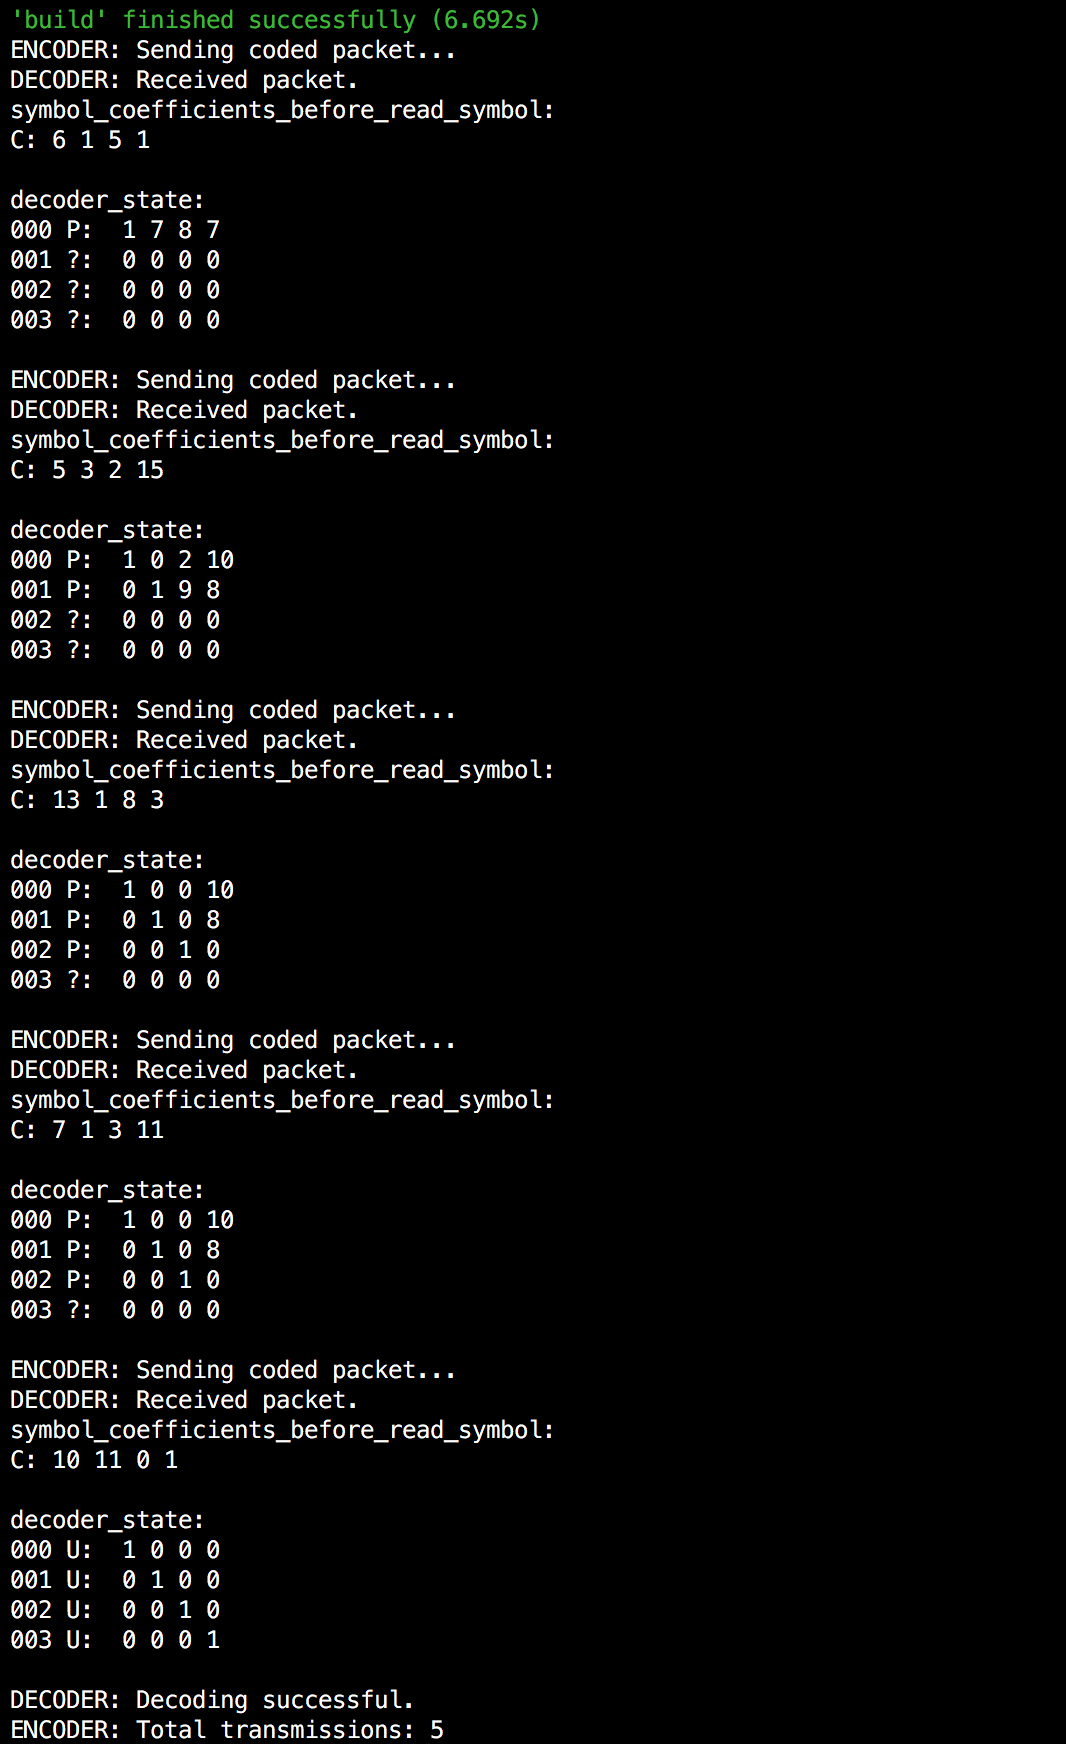
\includegraphics[scale=0.7]{figs/trace}}
	\caption{A trace of the encoder and decoder operations in an ns-3 simulation of my network coding protocol.}
	\label{fig:trace}
\end{figure}



\end{document}
